\documentclass[12pt,ngerman,bibtotoc]{scrreprt}

\usepackage[utf8]{inputenc}
\usepackage[T1]{fontenc}
\usepackage{booktabs}
\usepackage{babel}
\usepackage{graphicx}
\usepackage{csquotes}
\usepackage{paralist}
\usepackage{xcolor}
\usepackage{blindtext}

\setlength{\parindent}{0pt}

\author{Uwe Ziegenhagen}
\title{Hallo Welt}

\def\bild{\rule{14cm}{10cm}}

\begin{document}

\begin{titlepage}
{\huge \textbf{FernUni Hagen \\
Lehrstuhl für Informatik}}\vspace{4cm}

\begin{center}
{\Huge \textbf{Hallo Welt! -- ein Satz, den \\ alle kennen}}
\end{center}\vspace{4cm}

\hspace{2cm}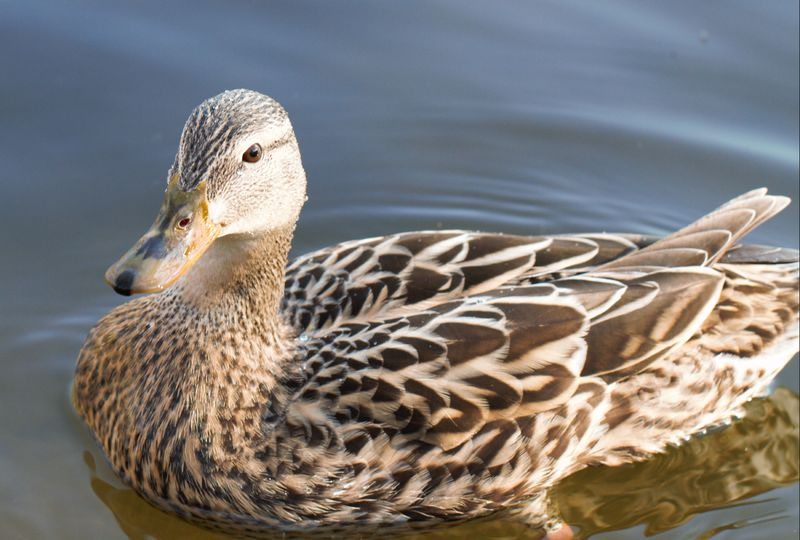
\includegraphics[width=5cm]{Bilder/image1}

\hfill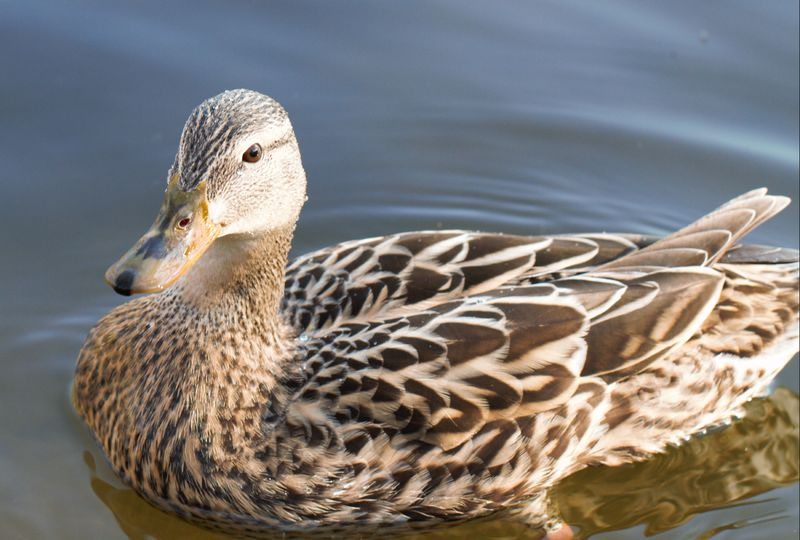
\includegraphics[width=5cm]{Bilder/image1}


\vfill
{\Large\textbf{1. Prüfer: Prof. Dr. Max Mustermann \\
2. Prüfer: Prof. Dr. Maria Mustermann}}
\end{titlepage}

\tableofcontents

\listoffigures

\chapter{Einleitung}\label{cha:einleitung}

\begin{quote}
\enquote{Hallo Welt!}
\end{quote}

\section{Hallo}

\blindtext[1]

\begin{figure}[h]
\begin{center}
\bild
\caption{Mein Bild}
\end{center}
\end{figure}

\blindtext[10]


\section{Halflo}

\blindtext[10]

\chapter{Hauptteil}

\section{Halqwlo}

\blindtext[10]

\section{Hakhllo}

\blindtext[10]


\chapter{Fazit}

\section{Hhkhallo}\label{sec:sonstwas}

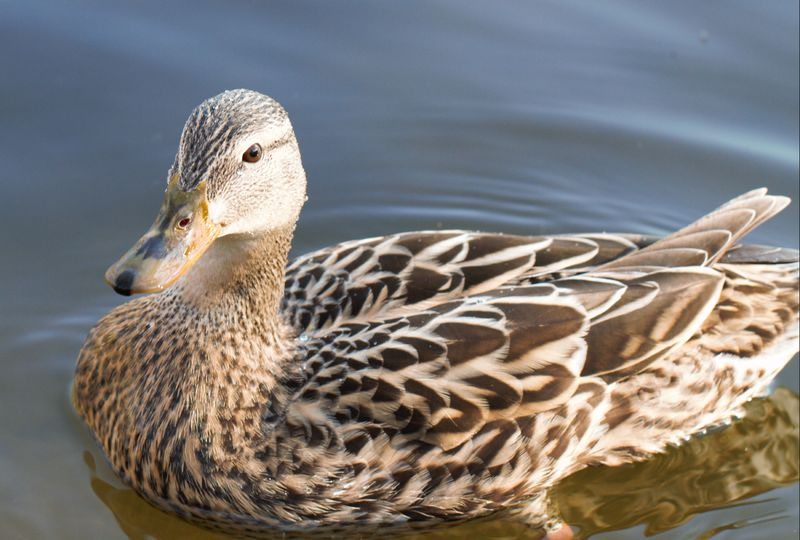
\includegraphics[width=\textwidth]{Bilder/image1}
\captionof{figure}{Hallo Welt2}


\blindtext[10]

\section{Hwerallo}

\blindtext[10]

\begin{equation}
a^2+b^2=c^2
\end{equation}

Siehe Kapitel \ref{cha:einleitung} und Abschnitt \ref{sec:sonstwas}

\end{document}